\chapter{Metodología}
\label{sec:metodologia}

En esta capítulo se detallará la metodología utilizada para alcanzar los objetivos del proyecto.

\section{Desarrollo incremental}
Este método consiste en una serie de iteraciones, en ventanas de tiempo, en las que al final de las mismas tendremos una parte del producto que el cliente podrá revisar y posteriormente mejorar y/o corregir [\cref{fig:metologia}]

\begin{figure}[htbp!]
    \centering
    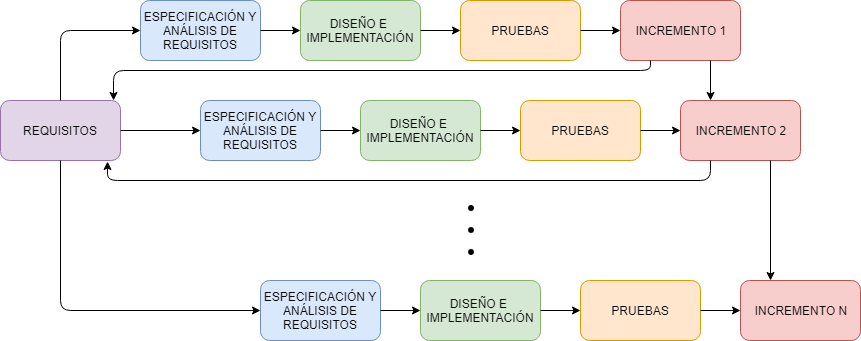
\includegraphics[width=\textwidth, keepaspectratio]{images/arquitectura/metodologia.png}
    \caption{Fases del modelo incremental}
    \label{fig:metologia}
\end{figure}

Esta metodología exige tener dos grupos de usuarios:

\begin{itemize}[noitemsep]
    \item \textbf{Cliente\footnote{Al ser un proyecto de fin de máster, no existe un cliente como tal, por lo que se ha decidido que los directores del proyecto tomen el rol de clientes.}:} Se encarga de revisar el producto al final de las iteraciones.
    \item \textbf{Desarrollador:} Se encarga de desarrollar el producto.
\end{itemize}


Las principales razones por las que se ha elegido esta metodología frente a otras existentes son:

\begin{itemize}[noitemsep]
    \item \textbf{El cliente no sabe exactamente lo que necesita:} Al inicio del proyecto se tenía una idea general del proyecto pero al tratarse de un proyecto con tantas partes diferenciadas los cambios, tecnologías, conexiones~\dots podrían sufrir cambios que implicasen redefinir ciertos conceptos.

    \item \textbf{Obtener un producto usable:} Este proyecto tiene una parte crítica, la de obtener el conjunto de datos lo más rápido posible. Esta parte implica tener una aplicación y el sistema de guardado de información lo antes posible para no bloquear el proyecto.
\end{itemize}

\section{Iteraciones}
El proyecto se dividió en varias iteraciones, en las cuales cada una de ellas proporciona una nueva funcionalidad del sistema.

\subsection{Iteración 0: Búsqueda de información sobre el dominio}
\subsection{Iteración 1: Sistema de captura de información}
\subsection{Iteración 2: Sistema de gestión de colas}
\subsection{Iteración 3: Sistema para el almacenamiento de la información}
\subsection{Iteración 4: Aplicación web de administración}
\subsection{Iteración 5: Comunicación aplicaciones y servidor}
\subsection{Iteración 6: Implementación de la Inteligencia Artificial}
\subsection{Iteración 7: Implementación de máquinas de Inteligencia Artificial}
\subsection{Iteración 8: Automatización del proceso de generación de modelos}

